\documentclass{PDS}

\usepackage{graphicx}
\usepackage{caption}
\usepackage{subcaption}

\usepackage{amsmath}
\usepackage{amssymb}
\usepackage{amsfonts}
\usepackage{amsthm}

\usepackage[round]{natbib}

\usepackage{newtxtext}
\usepackage{newtxmath}

\usepackage{xcolor}
\usepackage[colorlinks,allcolors=dscolor,bookmarks=false]{hyperref}

\jyear{2025}
\jdoi{https://doi.org/10.1017/pds.2025.xxx}

\begin{document}

\title{First experiences from using CADdrive in education}

\author{Georg Hackenberg}
\author{Christian Zehetner}

\address{School of Engineering, University of Applied Sciences Upper Austria, 4600 Wels, Austria}

\corresemail{georg.hackenberg@fh-wels.at}

\abstract{
    TODO
}

\keywords{product design, systems engineering, engineering education}

\maketitle

\section{Introduction}
\label{sec:introduction}

TODO~\cite{Hackenberg_2023}

\paragraph{Research question}

TODO

\paragraph{Contribution}

Section~\ref{sec:contribution}.
Section~\ref{sec:discussion}.
Section~\ref{sec:conclusion}.

\section{Course formats}
\label{sec:contribution}

TODO

\begin{enumerate}
    \item Project course on product design with Master students
    \item Course on systems engineering with Master students
    \item Workshop on product design with children
\end{enumerate}

TODO

\subsection{Project course on product design with Master students}

TODO

\begin{figure}[htbp]
    \centering
    \begin{subfigure}[b]{0.3\textwidth}
        \centering
        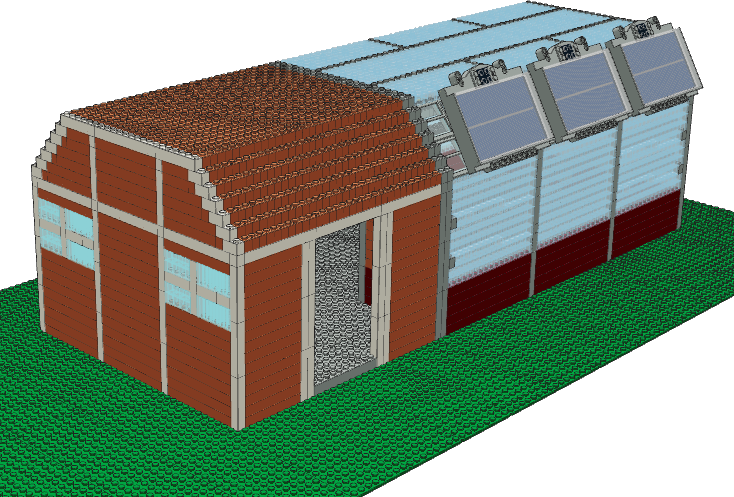
\includegraphics[width=\textwidth]{./figures/glasshouse_1.png}
        \caption{Exterior design}
        \label{fig:glasshouse_1}
    \end{subfigure}
    \hfill
    \begin{subfigure}[b]{0.3\textwidth}
        \centering
        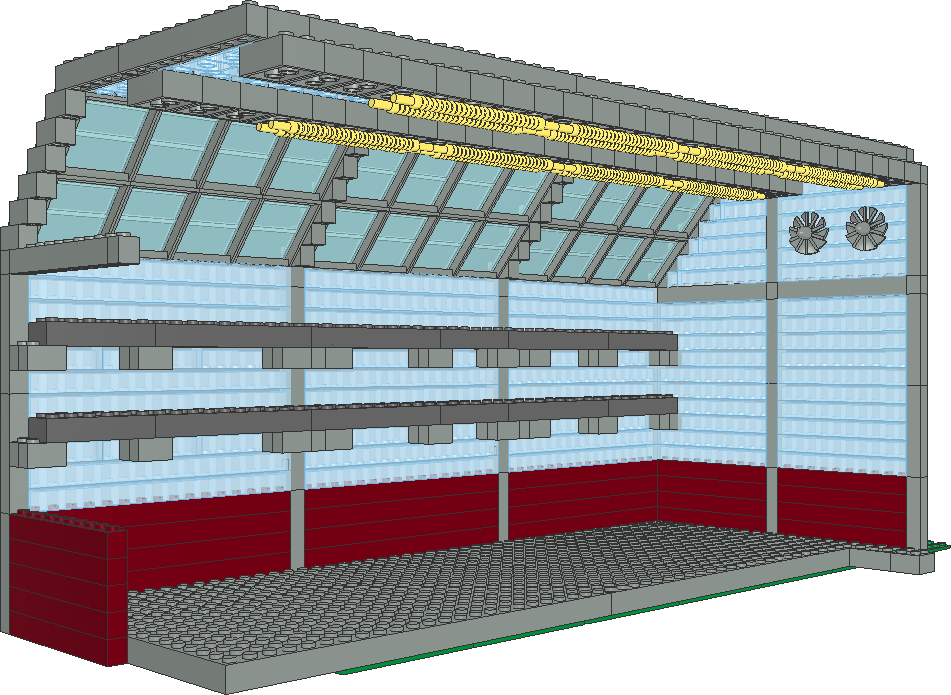
\includegraphics[width=\textwidth]{./figures/glasshouse_2.png}
        \caption{Interior design (grow area)}
        \label{fig:glasshouse_2}
    \end{subfigure}
    \hfill
    \begin{subfigure}[b]{0.3\textwidth}
        \centering
        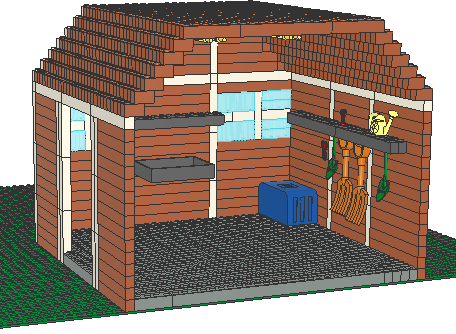
\includegraphics[width=\textwidth]{./figures/glasshouse_3.png}
        \caption{Interior design (shed area)}
        \label{fig:glasshouse_3}
    \end{subfigure}
    \caption{Mechanical design.}
    \label{fig:glasshouse}
\end{figure}

TODO

\begin{figure}[htbp]
    \begin{subfigure}[b]{0.56\textwidth}
        \centering
        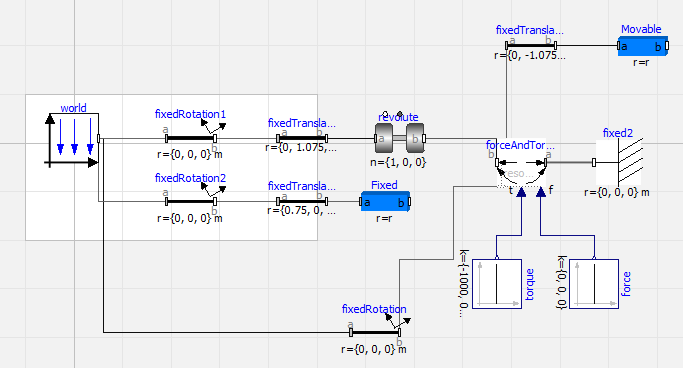
\includegraphics[width=\textwidth]{./figures/glasshouse_mechatronic_1.png}
        \caption{Component model}
    \end{subfigure}
    \hfill
    \begin{subfigure}[b]{0.4\textwidth}
        \centering
        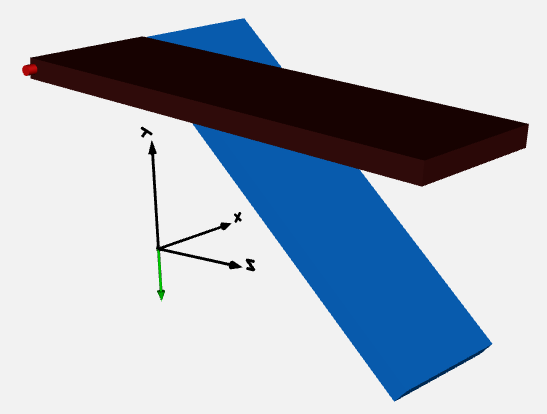
\includegraphics[width=\textwidth]{./figures/glasshouse_mechatronic_2.png}
        \caption{3D visualization}
    \end{subfigure}
    \caption{Mechatronic simulation.}
\end{figure}

\subsection{Course on systems engineering with Master students}

TODO

\begin{figure}[htbp]
    \centering
    \begin{subfigure}[b]{0.3\textwidth}
        \centering
        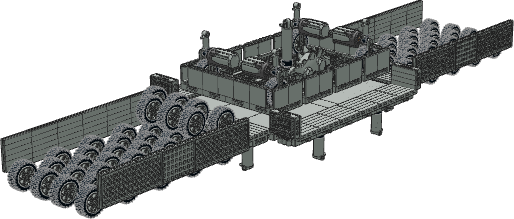
\includegraphics[width=\textwidth]{./figures/paper_1.png}
        \caption{First group}
        \label{fig:paper_1}
    \end{subfigure}
    \hfill
    \begin{subfigure}[b]{0.3\textwidth}
        \centering
        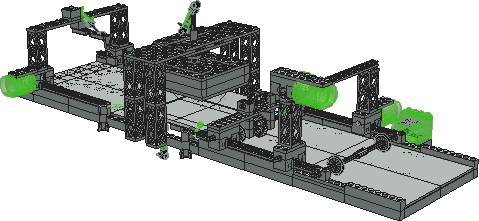
\includegraphics[width=\textwidth]{./figures/paper_2.png}
        \caption{Second group}
        \label{fig:paper_2}
    \end{subfigure}
    \hfill
    \begin{subfigure}[b]{0.3\textwidth}
        \centering
        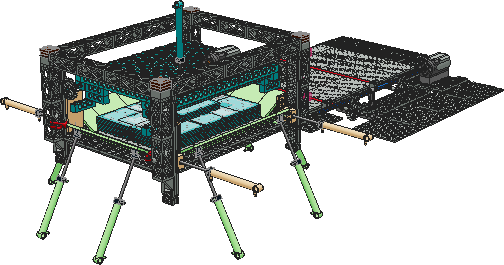
\includegraphics[width=\textwidth]{./figures/paper_3.png}
        \caption{Third group}
        \label{fig:paper_3}
    \end{subfigure}
    \caption{Mechanical designs}
    \label{fig:paper}
\end{figure}

TODO

\begin{figure}[htbp]
    \centering
    \begin{subfigure}[b]{0.45\textwidth}
        \centering
        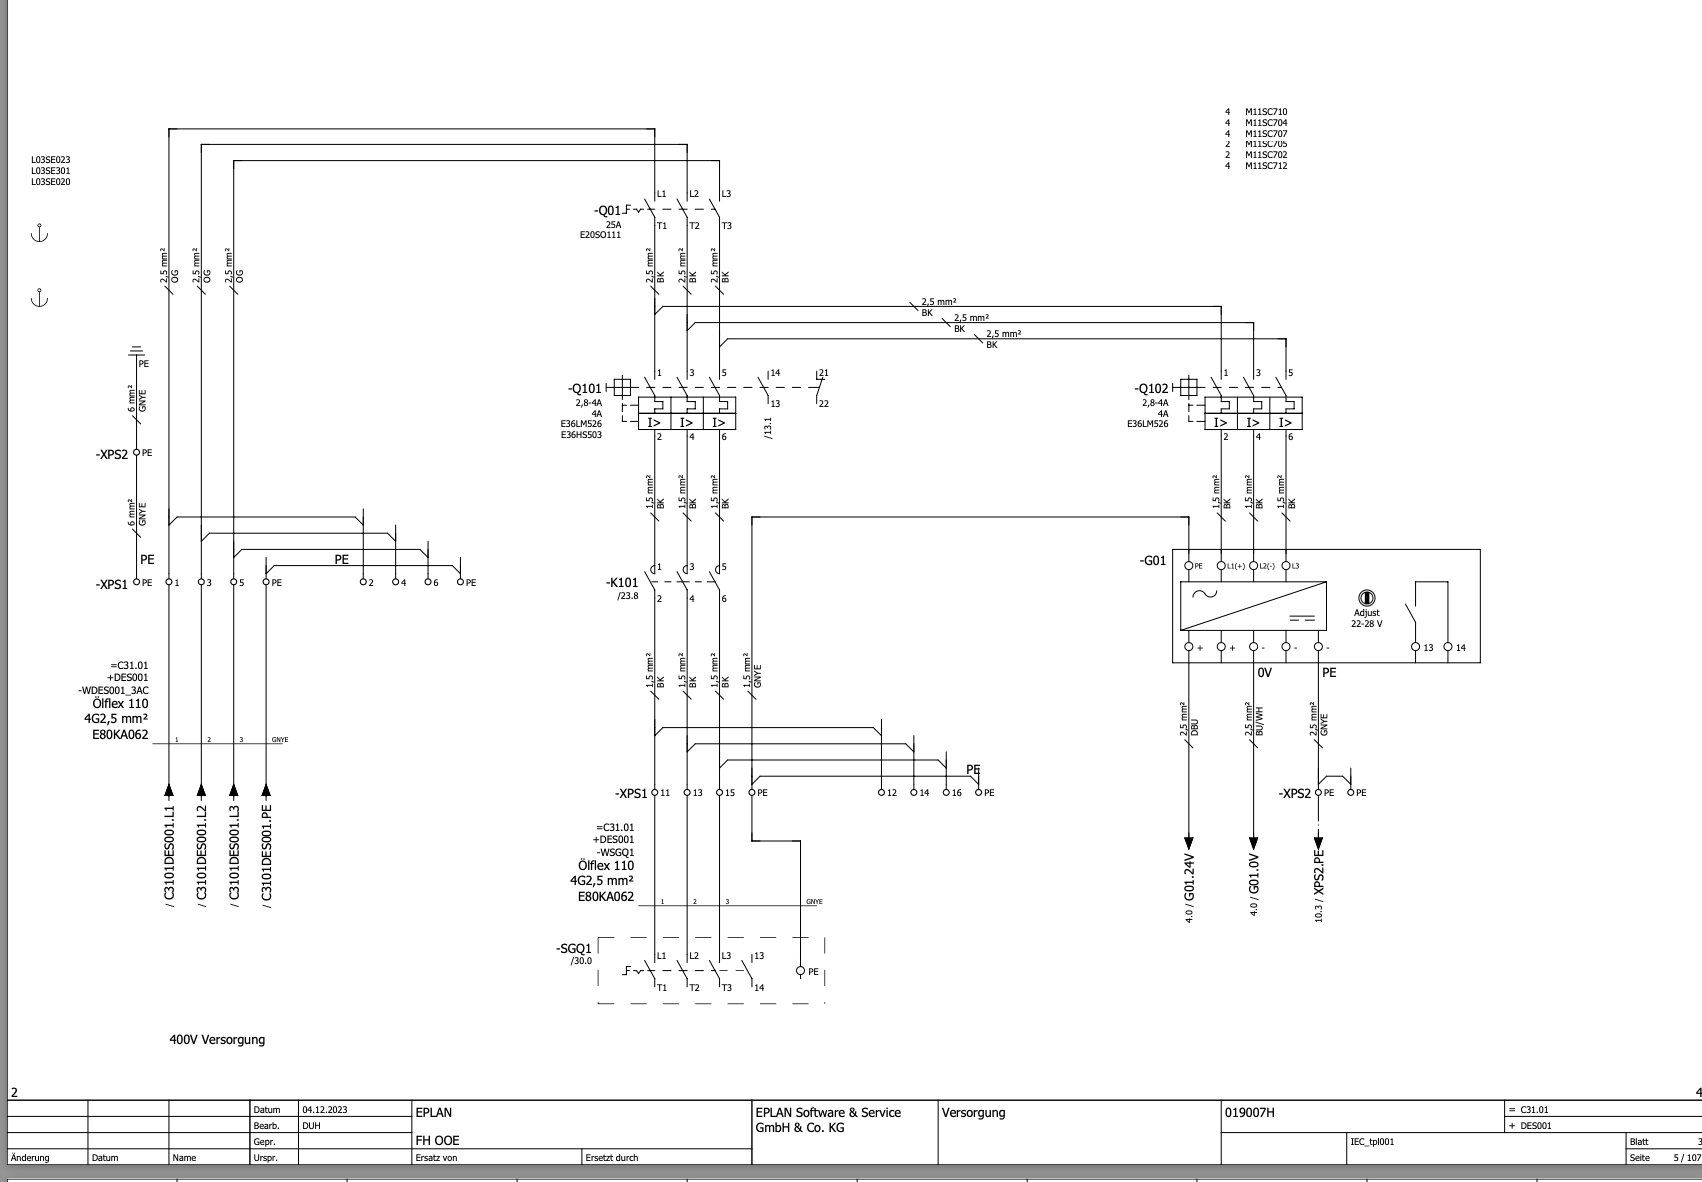
\includegraphics[width=\textwidth]{./figures/paper_electric.png}
        \caption{Electrical design}
    \end{subfigure}
    \hfill
    \begin{subfigure}[b]{0.5\textwidth}
        \centering
        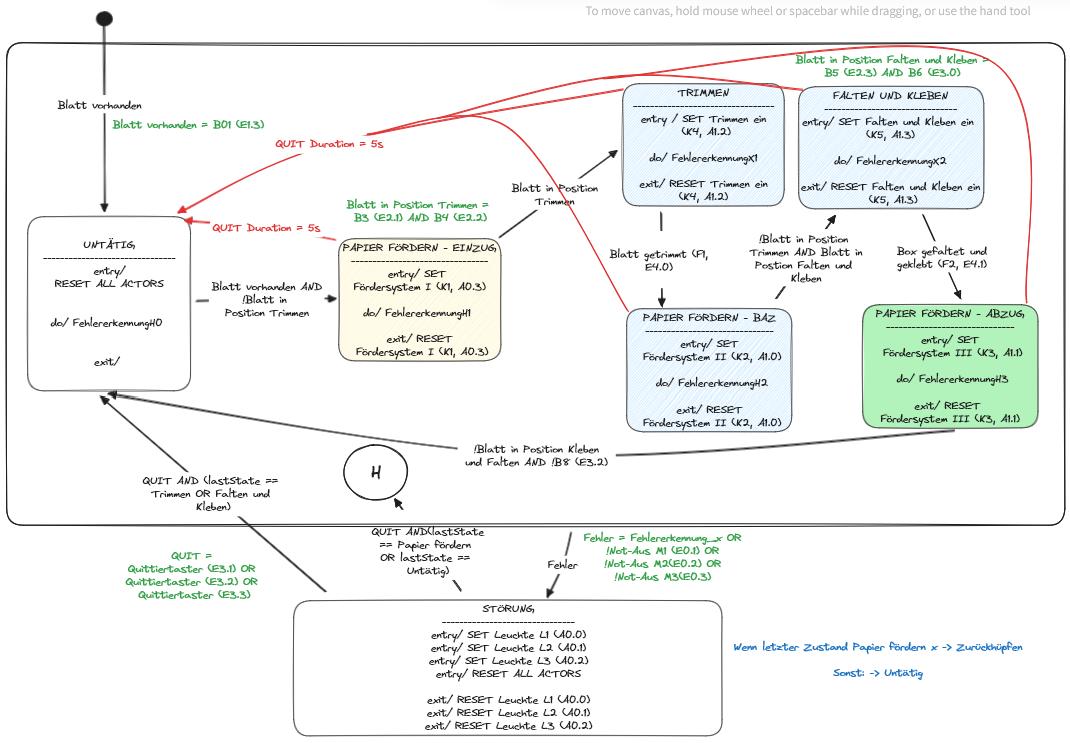
\includegraphics[width=\textwidth]{./figures/paper_control.png}
        \caption{Logical design}
    \end{subfigure}
    \caption{Electrical and logical designs.}
\end{figure}

TODO

\subsection{Workshop on product design with children}

TODO

\begin{figure}[htbp]
    \centering
    \begin{subfigure}[b]{0.3\textwidth}
        \centering
        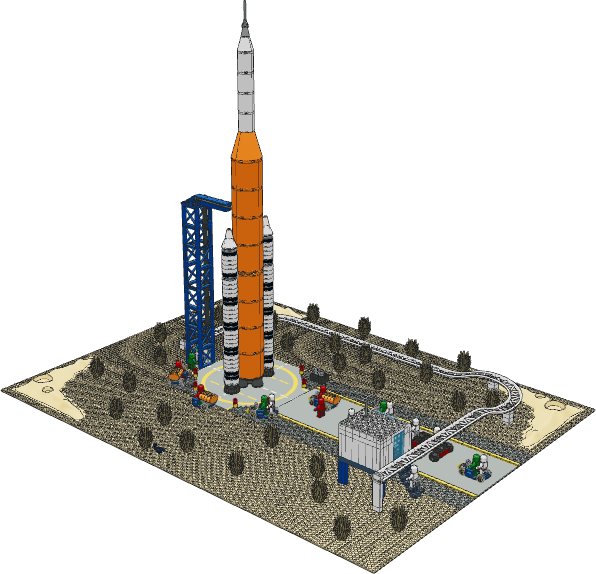
\includegraphics[width=\textwidth]{./figures/space.png}
        \caption{Space station}
        \label{fig:rocket}
    \end{subfigure}
    \hfill
    \begin{subfigure}[b]{0.3\textwidth}
        \centering
        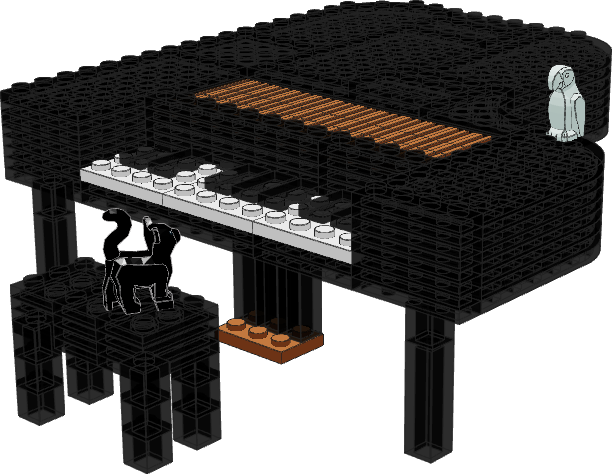
\includegraphics[width=\textwidth]{./figures/piano.png}
        \caption{Animal piano}
        \label{fig:piano}
    \end{subfigure}
    \hfill
    \begin{subfigure}[b]{0.3\textwidth}
        \centering
        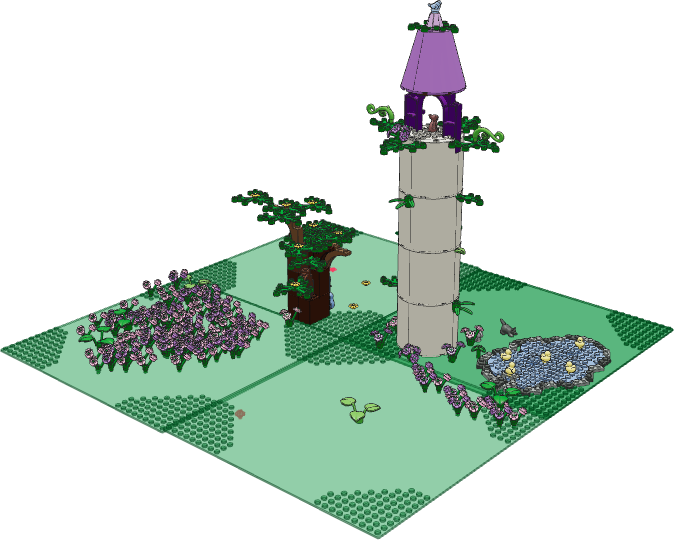
\includegraphics[width=\textwidth]{./figures/rapunzel.png}
        \caption{Rapunzel tower}
        \label{fig:rapunzel}
    \end{subfigure}
    \caption{Product designs.}
    \label{fig:kinderuni}
\end{figure}

TODO

\begin{figure}[htbp]
    \begin{subfigure}[b]{0.3\textwidth}
        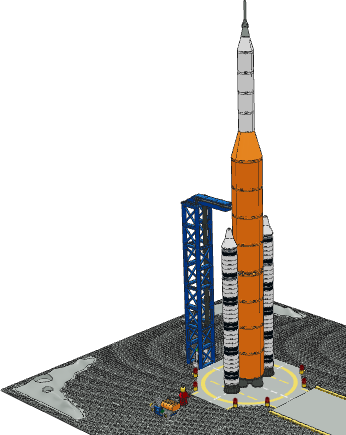
\includegraphics[width=\textwidth]{./figures/space_rocket.png}
        \caption{Rocket}
    \end{subfigure}
    \hfill
    \begin{subfigure}[b]{0.65\textwidth}
        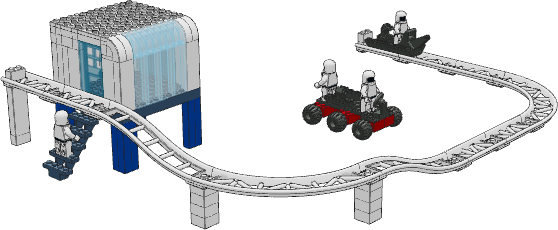
\includegraphics[width=\textwidth]{./figures/space_station.png}
        \caption{Station}
    \end{subfigure}
    \caption{Product components.}
\end{figure}

TODO

\section{Discussion}
\label{sec:discussion}

TODO

\section{Conclusion}
\label{sec:conclusion}

TODO

\paragraph{Summary}

TODO

\paragraph{Outlook}

TODO

\begin{Backmatter}

\bibliography{main}
\bibliographystyle{plainnat}

\end{Backmatter}

\end{document}